%%%%%%%%%%%%%%%%%%%%%%%%%%%%%%%%%%%%%%%%%
% Programming/Coding Assignment
% LaTeX Template
%
% This template has been downloaded from:
% http://www.latextemplates.com
%
% Original author:
% Ted Pavlic (http://www.tedpavlic.com)
%
% Note:
% The \lipsum[#] commands throughout this template generate dummy text
% to fill the template out. These commands should all be removed when 
% writing assignment content.
%
% This template uses a Perl script as an example snippet of code, most other
% languages are also usable. Configure them in the "CODE INCLUSION 
% CONFIGURATION" section.
%
%%%%%%%%%%%%%%%%%%%%%%%%%%%%%%%%%%%%%%%%%

%----------------------------------------------------------------------------------------
%	PACKAGES AND OTHER DOCUMENT CONFIGURATIONS
%----------------------------------------------------------------------------------------

\documentclass{article}

\usepackage{fancyhdr} % Required for custom headers
\usepackage{lastpage} % Required to determine the last page for the footer
\usepackage{extramarks} % Required for headers and footers
\usepackage[usenames,dvipsnames]{color} % Required for custom colors
\usepackage{graphicx} % Required to insert images
\usepackage{listings} % Required for insertion of code
\usepackage{courier} % Required for the courier font
\usepackage{lipsum} % Used for inserting dummy 'Lorem ipsum' text into the template
\usepackage{tocloft}
\usepackage{amsmath}

% Margins
\topmargin=-0.45in
\evensidemargin=0in
\oddsidemargin=0in
\textwidth=6.5in
\textheight=9.0in
\headsep=0.25in

\linespread{1.1} % Line spacing

% Set up the header and footer
\pagestyle{fancy}
\lhead{\hmwkTitle\ (\hmwkClassTime)} % Top center head
\renewcommand{\sectionmark}[1]{\markright{#1}}
\rhead{\rightmark} % Top right header
\lfoot{\lastxmark} % Bottom left footer
\cfoot{} % Bottom center footer
\rfoot{\thepage\ /\ \protect\pageref{LastPage}} % Bottom right footer
\renewcommand\headrulewidth{0.4pt} % Size of the header rule
\renewcommand\footrulewidth{0.4pt} % Size of the footer rule

\setlength\parindent{25pt} % Removes all indentation from paragraphs

%----------------------------------------------------------------------------------------
%	CODE INCLUSION CONFIGURATION
%----------------------------------------------------------------------------------------

\definecolor{MyDarkGreen}{rgb}{0.0,0.4,0.0} % This is the color used for comments
\lstloadlanguages{Perl} % Load Perl syntax for listings, for a list of other languages supported see: ftp://ftp.tex.ac.uk/tex-archive/macros/latex/contrib/listings/listings.pdf
\lstset{language=Perl, % Use Perl in this example
	frame=single, % Single frame around code
	basicstyle=\small\ttfamily, % Use small true type font
	keywordstyle=[1]\color{Blue}\bf, % Perl functions bold and blue
	keywordstyle=[2]\color{Purple}, % Perl function arguments purple
	keywordstyle=[3]\color{Blue}\underbar, % Custom functions underlined and blue
	identifierstyle=, % Nothing special about identifiers                                         
	commentstyle=\usefont{T1}{pcr}{m}{sl}\color{MyDarkGreen}\small, % Comments small dark green courier font
	stringstyle=\color{Purple}, % Strings are purple
	showstringspaces=false, % Don't put marks in string spaces
	tabsize=5, % 5 spaces per tab
	%
	% Put standard Perl functions not included in the default language here
	morekeywords={rand},
	%
	% Put Perl function parameters here
	morekeywords=[2]{on, off, interp},
	%
	% Put user defined functions here
	morekeywords=[3]{test},
	%
	morecomment=[l][\color{Blue}]{...}, % Line continuation (...) like blue comment
	numbers=left, % Line numbers on left
	firstnumber=1, % Line numbers start with line 1
	numberstyle=\tiny\color{Blue}, % Line numbers are blue and small
	stepnumber=5 % Line numbers go in steps of 5
}

% Creates a new command to include a perl script, the first parameter is the filename of the script (without .pl), the second parameter is the caption
\newcommand{\perlscript}[2]{
	\begin{itemize}
		\item[]\lstinputlisting[caption=#2,label=#1]{#1.pl}
	\end{itemize}
}

%----------------------------------------------------------------------------------------
%	DOCUMENT STRUCTURE COMMANDS
%	Skip this unless you know what you're doing
%----------------------------------------------------------------------------------------

% Header and footer for when a page split occurs within a problem environment
\newcommand{\enterProblemHeader}[1]{
	\nobreak\extramarks{#1}{#1 continued on next page\ldots}\nobreak
	\nobreak\extramarks{#1 (continued)}{#1 continued on next page\ldots}\nobreak
}

% Header and footer for when a page split occurs between problem environments
\newcommand{\exitProblemHeader}[1]{
	\nobreak\extramarks{#1 (continued)}{#1 continued on next page\ldots}\nobreak
	\nobreak\extramarks{#1}{}\nobreak
}

\setcounter{secnumdepth}{0} % Removes default section numbers
\newcounter{homeworkProblemCounter} % Creates a counter to keep track of the number of problems

\newcommand{\homeworkProblemName}{}
\newenvironment{homeworkProblem}[1][Problem \arabic{homeworkProblemCounter}]{ % Makes a new environment called homeworkProblem which takes 1 argument (custom name) but the default is "Problem #"
	\stepcounter{homeworkProblemCounter} % Increase counter for number of problems
	\renewcommand{\homeworkProblemName}{#1} % Assign \homeworkProblemName the name of the problem
	\section{\homeworkProblemName} % Make a section in the document with the custom problem count
	\enterProblemHeader{\homeworkProblemName} % Header and footer within the environment
}{
\exitProblemHeader{\homeworkProblemName} % Header and footer after the environment
}

\newcommand{\problemAnswer}[1]{ % Defines the problem answer command with the content as the only argument
	\noindent\framebox[\columnwidth][c]{\begin{minipage}{0.98\columnwidth}#1\end{minipage}} % Makes the box around the problem answer and puts the content inside
}

\newcommand{\homeworkSectionName}{}
\newenvironment{homeworkSection}[1]{ % New environment for sections within homework problems, takes 1 argument - the name of the section
	\renewcommand{\homeworkSectionName}{#1} % Assign \homeworkSectionName to the name of the section from the environment argument
	\subsection{\homeworkSectionName} % Make a subsection with the custom name of the subsection
	\enterProblemHeader{\homeworkProblemName\ [\homeworkSectionName]} % Header and footer within the environment
}{
\enterProblemHeader{\homeworkProblemName} % Header and footer after the environment
}

%----------------------------------------------------------------------------------------
%	NAME AND CLASS SECTION
%----------------------------------------------------------------------------------------

\newcommand{\hmwkTitle}{Eindverslag `Chips \& Circuits'} % Assignment title
\newcommand{\hmwkDueDate}{17-12-2015} % Due date
\newcommand{\hmwkClass}{Programmeertheorie, Groep D} % Course/class
\newcommand{\hmwkClassTime}{HaMaMa} % Class/lecture time
\newcommand{\hmwkClassInstructor}{docenten: Daan van den Berg, Jelle van Assema, Maarten Inja} % Teacher/lecturer
\newcommand{\hmwkAuthorName}{Maurits de Ridder, Hasine Efeturk, Marianne de Heer Kloots} % Your name

%----------------------------------------------------------------------------------------
%	TITLE PAGE
%----------------------------------------------------------------------------------------

\title{
	\vfill
	\textmd{\textbf{\hmwkTitle}}\\
	\vspace{0.1in}\large{\textit{\hmwkAuthorName}} \\
	\normalsize\vspace{0.1in}\small{\hmwkClass, `\hmwkClassTime'\\ \hmwkClassInstructor\\ \hmwkDueDate} \\
	\vfill \vfill \vfill
	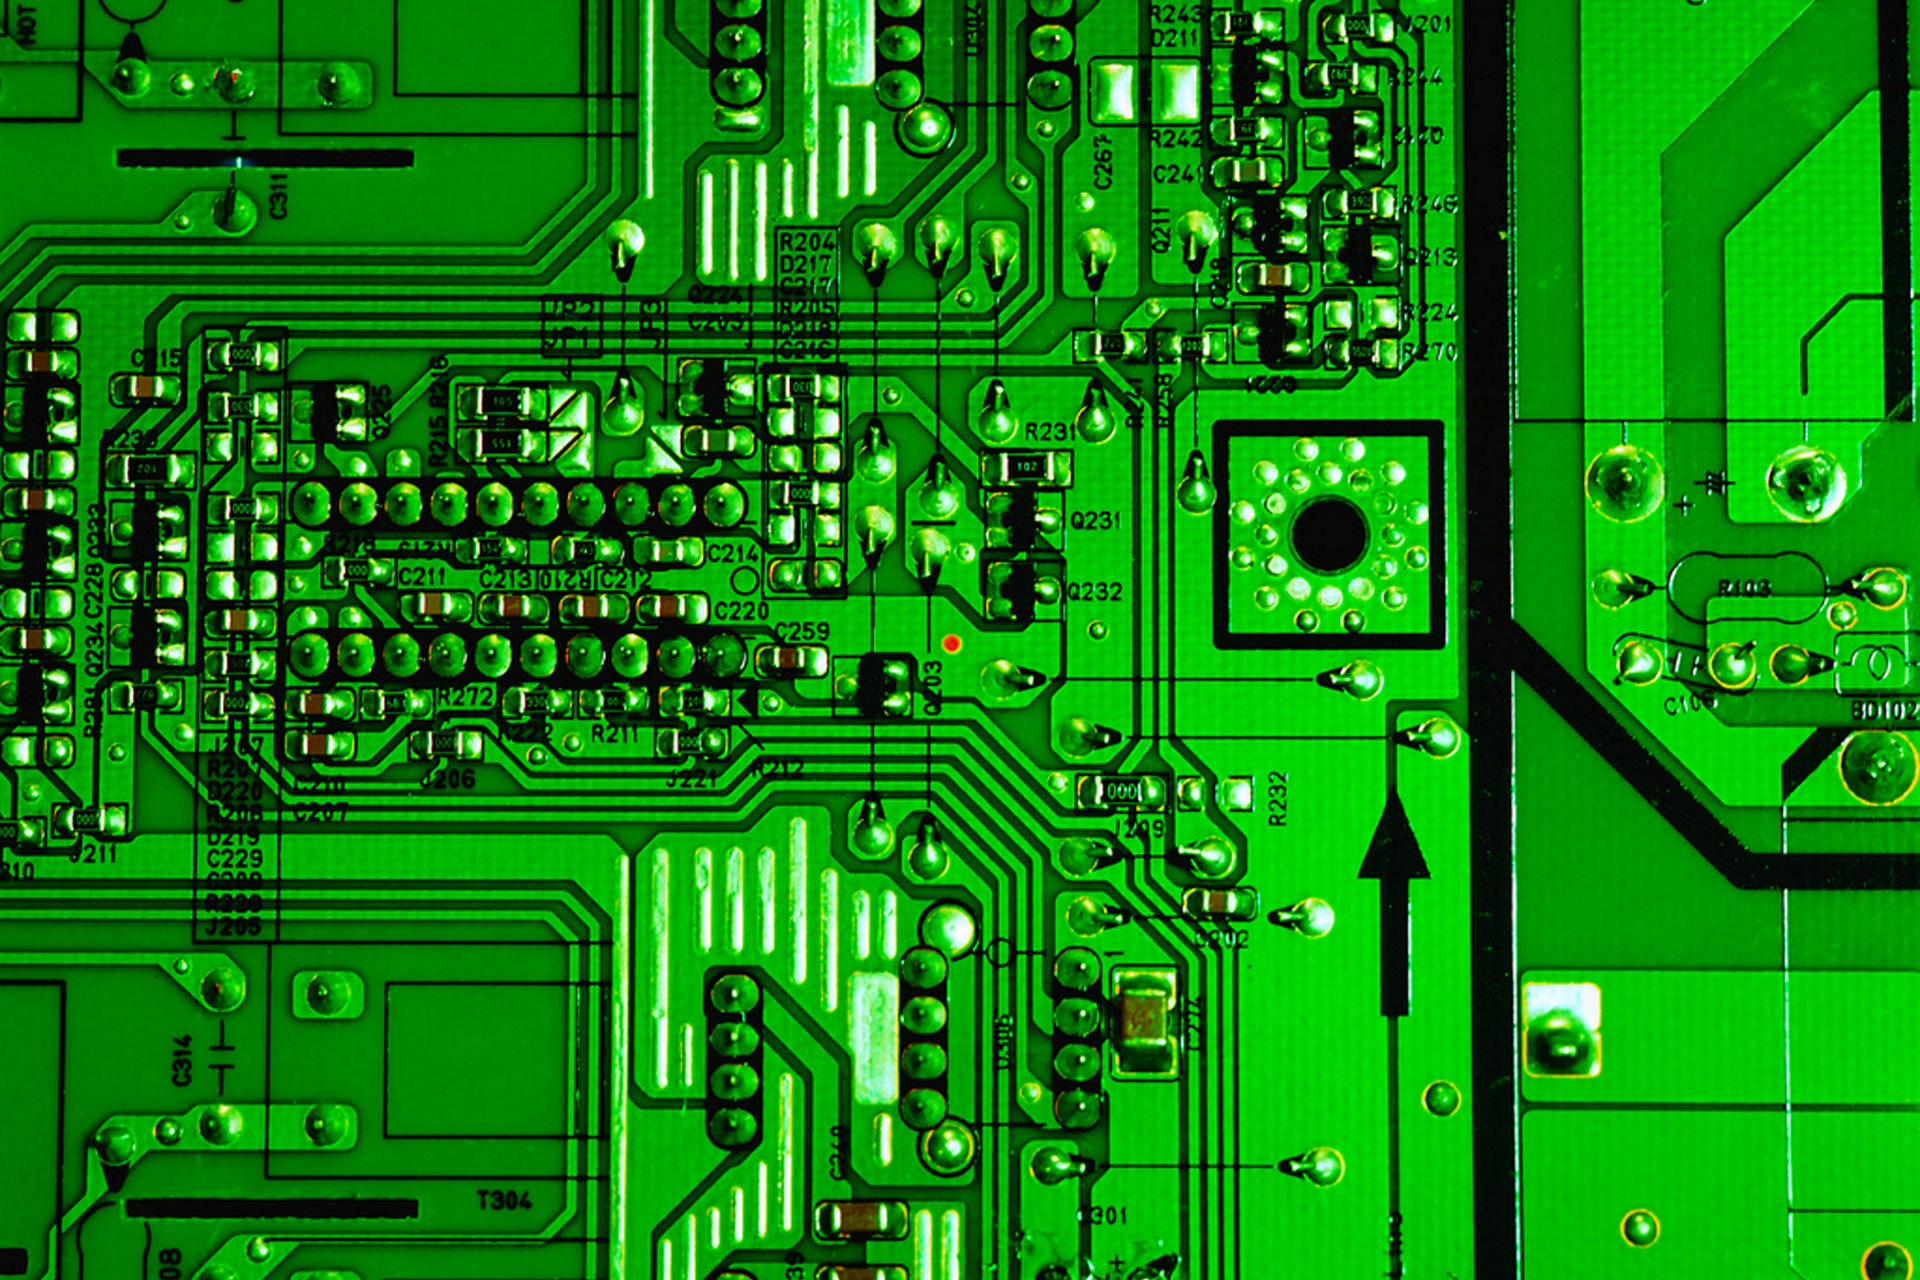
\includegraphics[width=0.75\columnwidth]{Circuit-board}
	\vfill
	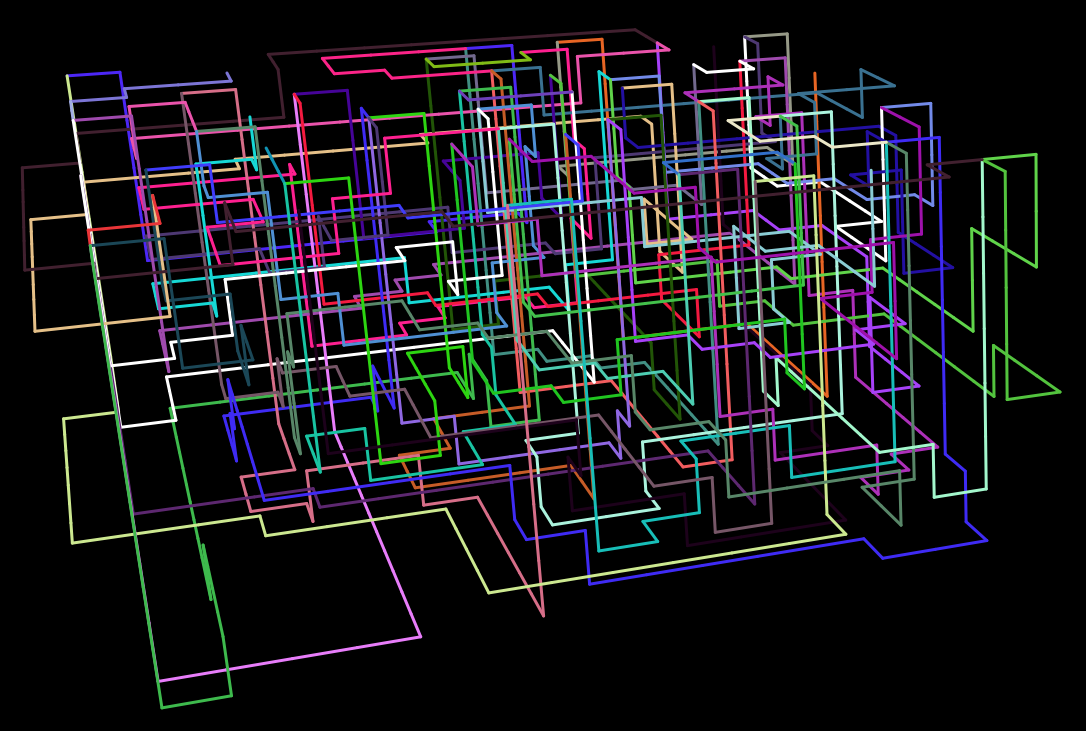
\includegraphics[width=0.75\columnwidth]{3dviz}
	\vfill
}

\date{} % Insert date here if you want it to appear below your name

%----------------------------------------------------------------------------------------

\begin{document}
	\pagenumbering{gobble}
	
	\maketitle
	
	%----------------------------------------------------------------------------------------
	%	TABLE OF CONTENTS
	%----------------------------------------------------------------------------------------
	
	%\setcounter{tocdepth}{1} % Uncomment this line if you don't want subsections listed in the ToC
	
	\newpage
	\pagenumbering{arabic}
	\renewcommand{\cftdot}{.}
	\renewcommand{\contentsname}{INHOUDSOPGAVE}
	\tableofcontents
	\newpage
	
	%----------------------------------------------------------------------------------------
	%	PROBLEM 1
	%----------------------------------------------------------------------------------------
	
	% To have just one problem per page, simply put a \clearpage after each problem

	\section{1. Inleiding}
	
	Elektronische chips (of \textit{ge\"\i ntegreerde circuits}) zijn te vinden in vrijwel elk elektronisch apparaat, van computers tot telefoons en magnetrons. Ze worden gebruikt om verschillende functies binnen deze apparaten uit te voeren, zoals het bijhouden van de tijd, maar ook bijvoorbeeld logische berekeningen. Computers kunnen met geen mogelijkheid zonder chips, en het optimaal configureren van deze chips is dus van essentieel belang. In dit verslag zullen we beschrijven hoe we de optimale configuratie van de circuits op een chip computationeel hebben proberen te simuleren, en de resultaten presenteren die daaruit zijn voortgekomen.
	\par
	Een chip bestaat uit een klein siliconen plaatje met een aantal logische gates, die op een gespecificeerde manier met elkaar zijn verbonden door elektrische paden. Een chip kan bestaan uit meerdere lagen, waarbij alleen op de bovenste laag gates zitten; de elektrische paden kunnen dan over meerdere lagen lopen. Voor onze simulatie hebben we twee verschillende chipconfiguraties gebruikt, met verschillende groottes en hoeveelheden gates. Voor beide configuraties konden de gates op drie verschillende manieren verbonden konden worden. De zes lijsten van met elkaar te verbinden gates noemen we netlists. De netlists specificeerden steeds een tiental van 30 tot 70 elektrische paden die gelegd moesten worden. De totale lengte van de paden moet zo kort mogelijk zijn, maar de te leggen paden mogen elkaar niet kruisen. Bovendien kunnen de paden uitwijken naar lagere lagen van de chip, maar in totaal kan de chip niet uit meer dan 8 lagen bestaan. ?? ZIE AFBEELDING ??
	\par
	De toestandsruimte met alle mogelijke paden is enorm: voor alleen alle mogelijke kortste paden bij de kleinste configuratie in onze simulatie (een chip van 18 bij 13 met 25 gates) is bijvoorbeeld al 1.763114 * 10105. Het beschreven probleem is daarom een NP-hard probleem - dat wil zeggen dat het niet in polynomiale tijd is op te lossen door middel van een brute force techniek (het simpelweg uitproberen van alle mogelijke opties). Het gebruik van slimme algoritmes en goed gekozen heuristieken is daarom belangrijk om toch binnen een redelijke tijd een werkbare oplossing te kunnen vinden.
	\par
	Voor onze simulatie hebben we verschillende zoekalgoritmen en heuristieken vergeleken. In het hoofdstuk ‘Methodes’ zullen we die bespreken en vergelijken. In de hoofdstukken ‘Resultaten’ en ‘Conclusie’ zullen we vervolgens onze beste resultaten presenteren en advies geven voor verdere mogelijke optimalisaties van chipconfiguraties.
	$\sum_{i=1}^{70} \frac{(|\Delta x[i]| + |\Delta y[i]|)!}{|\Delta x[i]|! * |\Delta y[i]|!} * 70!$
	
	
	
	\section{2. Methodes}
	
	\subsection{2.1 Vooraf: algoritmes}
	
	\subsubsection{2.1.1 BFS}
	
	\subsubsection{2.1.2 A*}
	
	\subsubsection{2.1.3 Netlists sorteren}
	Netlist ordenen kort-lang: 24,25,26; lang-kort 17-18
	
	\subsubsection{2.1.4 Kruisingen toestaan}
	
	\subsubsection{2.1.5 Loskoppelen gate-buren}
	
	\subsubsection{2.1.6 Toewijzing random layers}
	
	\subsection{2.2 Achteraf: optimalisatie}
	
	
	\subsection{Bla}
	
	Bla bla
	
	\subsection{Bla}
	
	Bla bla bla
	
	\section{Resultaten en conclusie}
	
	Bla!
	
\end{document}